\documentclass[french]{beamer}

\usepackage[utf8]{inputenc}
\usepackage[T1]{fontenc}
\usepackage[english,french]{babel}
\usepackage{graphicx}
\usepackage{amsmath}
\usepackage{fancyvrb}
\usepackage{listings}
\usepackage{color}
\usepackage{enumerate}
 
\definecolor{codegreen}{rgb}{0,0.6,0}
\definecolor{codegray}{rgb}{0.5,0.5,0.5}
\definecolor{codepurple}{rgb}{0.58,0,0.82}
\definecolor{backcolour}{rgb}{0.95,0.95,0.92}

\lstdefinestyle{mystyle}{
    backgroundcolor=\color{backcolour},   
    commentstyle=\color{codegreen},
    keywordstyle=\color{magenta},
    numberstyle=\tiny\color{codegray},
    stringstyle=\color{codepurple},
    basicstyle=\footnotesize,
    breakatwhitespace=false,         
    breaklines=true,                 
    captionpos=b,                    
    keepspaces=true,                 
    numbers=left,                    
    numbersep=5pt,                  
    showspaces=false,                
    showstringspaces=false,
    showtabs=false,                  
    tabsize=2
}

\lstset{language=C++,
    basicstyle=\small,
    keywordstyle=\color{blue}\small,
    stringstyle=\color{red}\small,
    commentstyle=\color{green}\small,
    morecomment=[l][\color{magenta}]{\#},
    tabsize=2
}

\definecolor{darkBlue}{RGB}{20,20,195}

\title{Projet Tétris}
\author{MAILLARD, ROYER, DILLON}
\date{13 mars 2019}


\usetheme{Madrid}
\useinnertheme{circles}
\usecolortheme{whale}


\begin{document}

\AtBeginSection[]{
	\begin{frame}{Plan}
		\tableofcontents[currentsection]
	\end{frame}
}


\begin{frame}

	\begin{columns}

		\hspace{-2.5cm}
		\begin{column}{0.2\textwidth}
			
\includegraphics[scale=0.3]{img/logU.png}
	
		\end{column}
		
		\begin{column}{0.2\textwidth}
			\vspace{0.1cm}
			
\includegraphics[scale=0.045]{img/logF.jpg}

		\end{column}

	\end{columns}

	\vspace{-0.15cm}

	\center{\textsc{\Huge \color{darkBlue} Le Vouitris}}

	\vspace{0.2cm}

	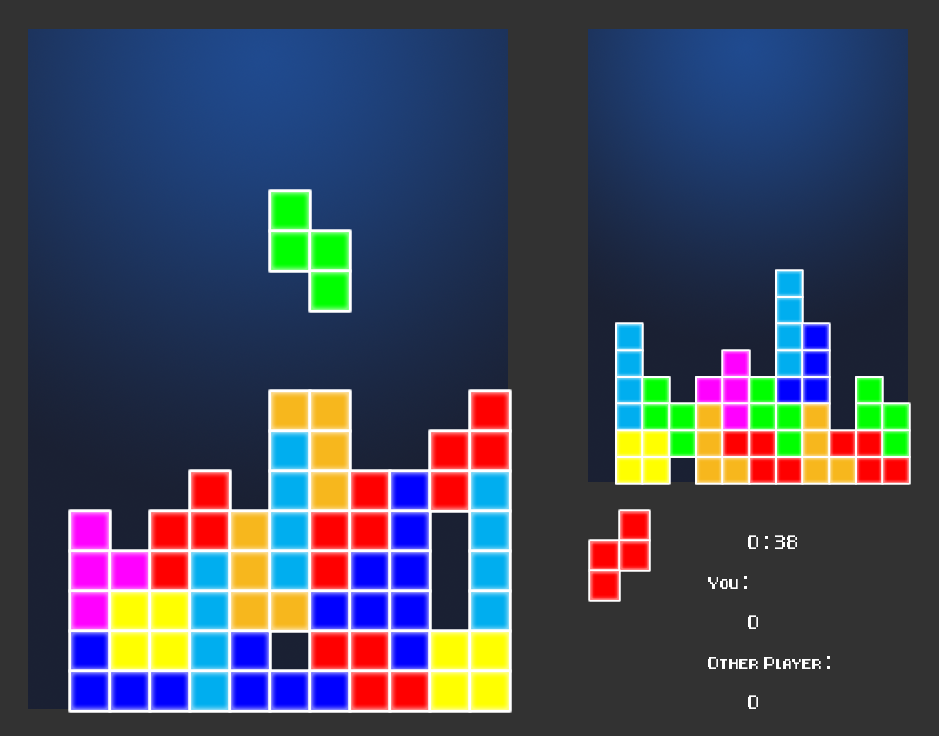
\includegraphics[scale=0.15]{img/vouitris.png}

	\center{\textsc{Cynthia MAILLARD, Félix ROYER, Alexandre DILLON}}
	\vspace{-0.20cm}
	
	\center{\textsc{\large 13 mars 2019}}

	\vspace{0.20cm}

	\textsc{\underline{Tuteur de projet} : Julien BERNARD}

\hspace{2cm}

\end{frame}

\begin{frame}{Plan}

	\tableofcontents

\end{frame}


\section{Adaptation du jeu d'origine}
	\subsection{Le jeu originel}

\begin{frame}{Adaptation du jeu d'origine}{Le jeu originel}

	\begin{block}{Le premier Tétris (1984) - Alekseï Pajitnov}
		\begin{itemize}
			\item jeu de puzzle
			\item succès mondial dans les années 1990
			\item adapté sur pratiquement toutes les consoles
			\item certaines versions multijoueurs
		\end{itemize}

	\end{block}

	\begin{center}
		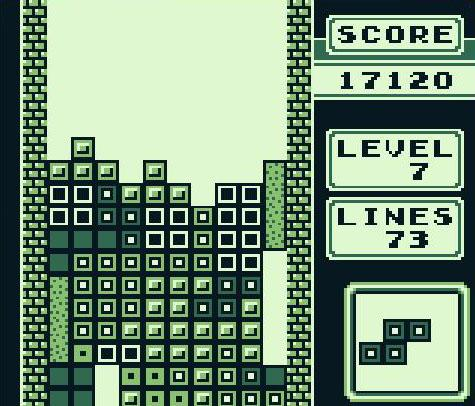
\includegraphics[scale=0.25]{img/Tetris8.jpg}
	\end{center}
\end{frame}


\begin{frame}{Adaptation du jeu d'origine}{Le jeu originel}
	\begin{block}{La jouabilité}
		\begin{itemize}
			\item déplacement latéral et rotation des tétrominos, chute accélerée des tétrominos
			\item agencer les tétrominos en ligne
			\item les lignes disparaissent, augmentant le score
			\item la partie s'arrête quand les tétrominos touchent le plafond
		\end{itemize}

	\end{block}

	\begin{center}
		
\includegraphics[scale=0.3]{img/1.png}
		
\includegraphics[scale=0.4]{img/2.png}
		
\includegraphics[scale=0.4]{img/3.png}
		
\includegraphics[scale=0.4]{img/4.png}
		
\includegraphics[scale=0.3]{img/5.png}
		
\includegraphics[scale=0.3]{img/6.png}
		
\includegraphics[scale=0.3]{img/7.png}
	\end{center}
\end{frame}

	\subsection{Notre adaptation}

\begin{frame}{Adaptation du jeu d'origine}{Notre adaptation}
	
	\begin{block}{Le cahier des charges}
		\begin{itemize}
			\item architecture client-serveur
			\item un joueur, un client, un ordinateur
			\item développement en C++ / Gamedev Framework / Boost::Asio
			\item développement de notre propre bibliothèque de sérialisation
		\end{itemize}
	\end{block}
	
	\begin{block}{Les objectifs}
		\begin{itemize}
			\item approfondir la programmation répartie
			\item établir un protocole réseau
			\item découvrir la sérialisation
			\item se familiariser aux bibliothèques graphiques
		\end{itemize}
	\end{block}

\end{frame}

\begin{frame}{Adaptation du jeu d'origine}{Notre adaptation}
	
	\begin{block}{Les choix d'implémentation}
		\begin{itemize}
			\item le serveur fait loi
			\item le client envoie les actions du joueur au serveur
			\item le serveur lui renvoie l'état du jeu mis à jour
			\item détruire des lignes inflige des malus à l'adversaire
			\begin{itemize}
				\item 1 ligne : pas de malus
				\item 2 lignes : empèche la rotation
				\item 3 lignes : accélération de la chute
				\item 4 lignes : suppression de blocs en bas du tableau
			\end{itemize}
		\end{itemize}
	\end{block}

	\begin{center}
		
\includegraphics[scale=0.2]{../ressources/malusNoRotate.png}
		
\includegraphics[scale=0.2]{../ressources/malusSpeed.png}
	\end{center}

\end{frame}

\begin{frame}{Adaptation du jeu d'origine}{Notre adaptation}
	\begin{block}{Les contrôles}
		\begin{itemize}
			\item $\gets$ : gauche
			\item $\to$ : droite
			\item $\downarrow$ : chute rapide
			\item \emph{SPACE} : rotation
		\end{itemize}
	\end{block}

\end{frame}


\section{Modélisation du jeu}
	\subsection{Architecture réseau}

		\begin{frame}{Modélisation du jeu}{Architecture réseau}
			\begin{center}
				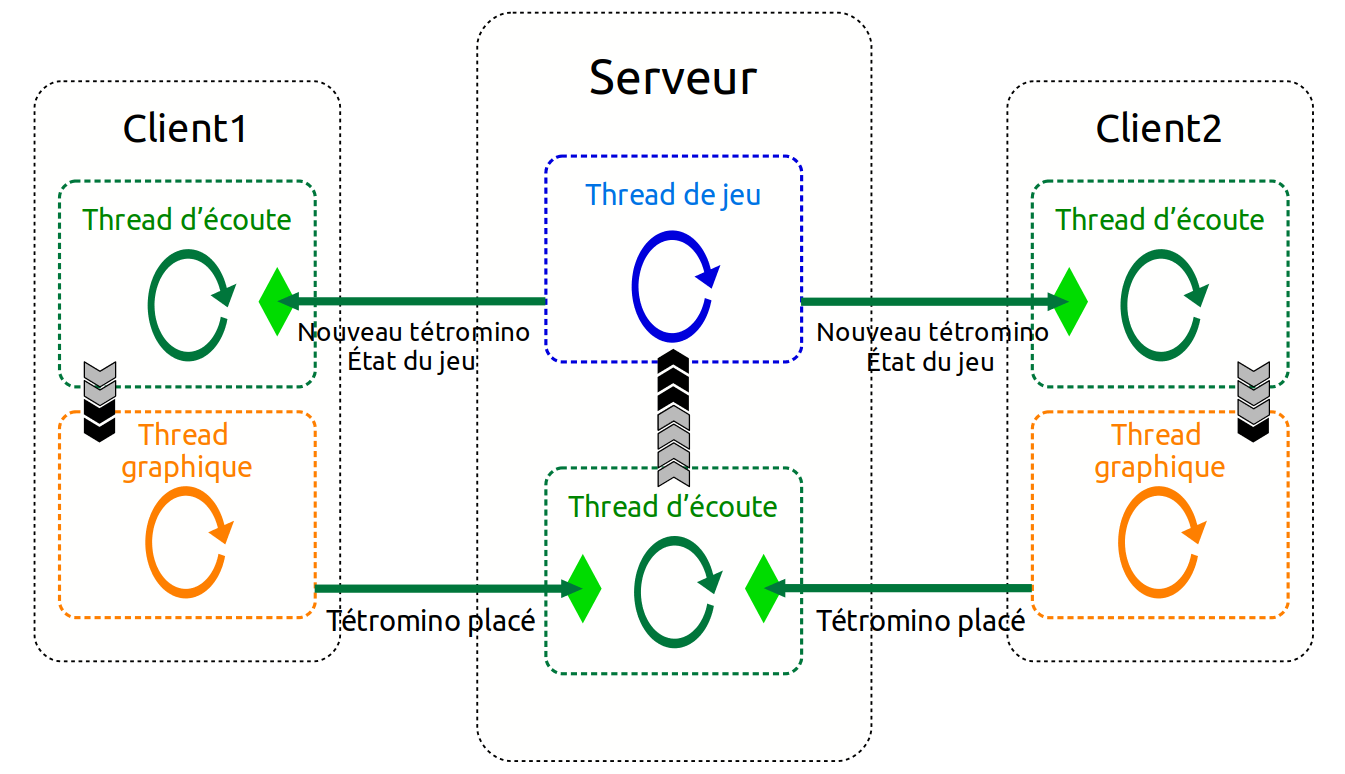
\includegraphics[scale=0.25]{img/archi_reseau.png}
			\end{center}
		\end{frame}

	\subsection{Protocole d'échange de messages}

		\begin{frame}{Modélisation du jeu}{Protocole d'échange de messages}
			\begin{center}
				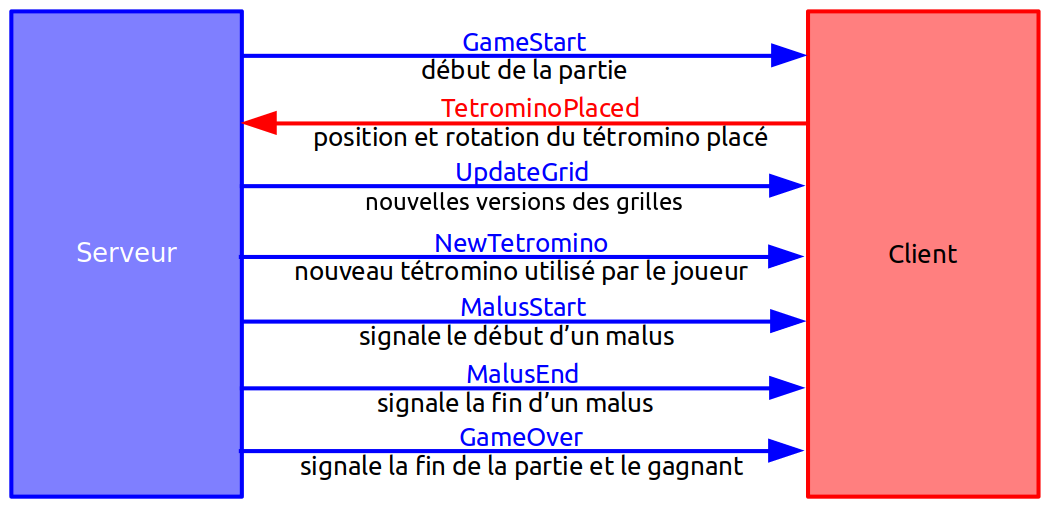
\includegraphics[scale=0.3]{img/ech.png}
			\end{center}
		\end{frame}

\section{La communication}

	\subsection{Le serveur}

	\begin{frame}{La communication}{Le serveur}
		\begin{columns}

			\begin{column}{0.4\textwidth}
				\begin{center}
					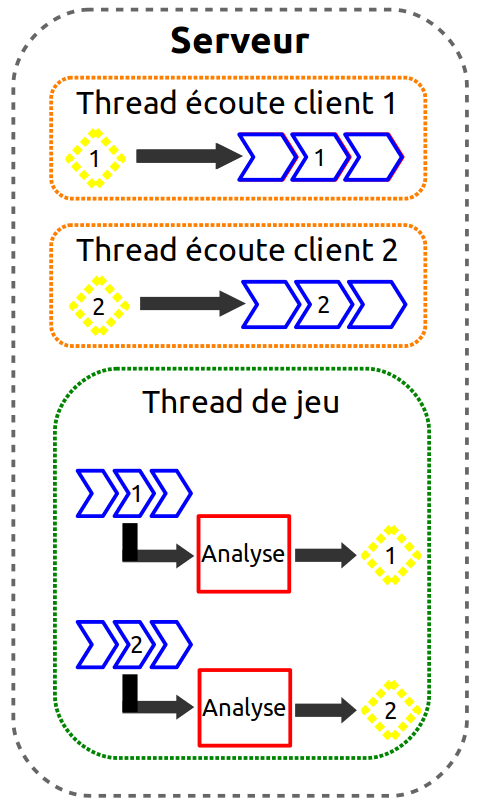
\includegraphics[scale=0.25]{img/serveur.png}
				\end{center}
			\end{column}


			\begin{column}{0.5\textwidth}

				\begin{block}{Les données contenues dans le serveur pour chacun des joueurs}
					\begin{itemize}
						\item grille de jeu
						\item score
						\item un vérificateur de triche
						\item un gestionnaire de malus
					\end{itemize}
				\end{block}

				\begin{center}
					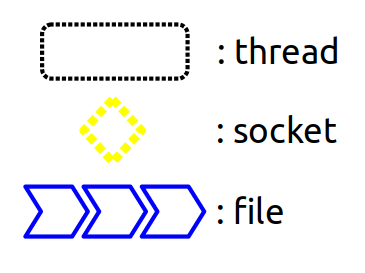
\includegraphics[scale=0.25]{img/legende.png}
				\end{center}

			\end{column}

		\end{columns}
	\end{frame}




	\begin{frame}{La communication}{Le serveur}
		\begin{block}{L'exploitation des messages}
			\begin{enumerate}
				\item{Reception message TetrominoPlaced}
				\item{Vérification triche}
				\item{Mise à jour de la grille}
				\item{Mise à jour du score}
				\item{Envoi de malus à l'adversaire}
				\item{Envoi grille mise à jour aux joueurs}
			\end{enumerate}
		\end{block}

	\end{frame}


	\begin{frame}{La communication}{Le serveur}
		\begin{block}{Le vérificateur de triche}
			\begin{itemize}
				\item Vérifie que les données renvoyées par le client sont cohérentes
				\begin{itemize}
					\item Le temps pour jouer la pièce n'est pas trop long
					\item Les malus sont bien appliqués
				\end{itemize}
				\item Trois fautes autorisées
			\end{itemize}
		\end{block}


	\end{frame}
























	\subsection{La sérialisation}

		\begin{frame}{La communication}{La sérialisation}
	        \begin{block}{Objectif}
	            Permettre les échanges de structures complexes entre clients et serveur via des messages standardisés.
	        \end{block}

	        \begin{block}{Modèles}
	            \begin{itemize}
	                \item GamedevFramework
	                \item SFML/Packet
	            \end{itemize}
	        \end{block}

	        \begin{block}{Structures de sérialisation}
	            Deux classes symétriques communes aux clients et au serveur : 
	            \begin{itemize}
	                \item Serializer
	                \item Deserializer
	            \end{itemize}
	        \end{block}     

	    \end{frame}

		\begin{frame}{La communication}{La sérialisation}
	        \begin{columns}
		        \begin{column}{0.65\textwidth}
			    	\begin{block}{Sérialisation templatée}
			            Utilisation d'une méthode templatée pour sérialiser tout type simple.

			        \end{block}
			        
			         \begin{block}{Endianess}
			            Ordre séquentiel dans lequel sont ranger nos données sérialisées.
			            \newline Endianess de format Big-Endian : par défaut sur les structures réseaux.
			        \end{block}

			       	\begin{block}{Sérialisation d'objet}
			            Sérialisation des attributs de l'objet que l'on souhaite communiquer.
			        \end{block}
				\end{column}

				\begin{column}{0.25\textwidth}
			        \begin{center}
			        	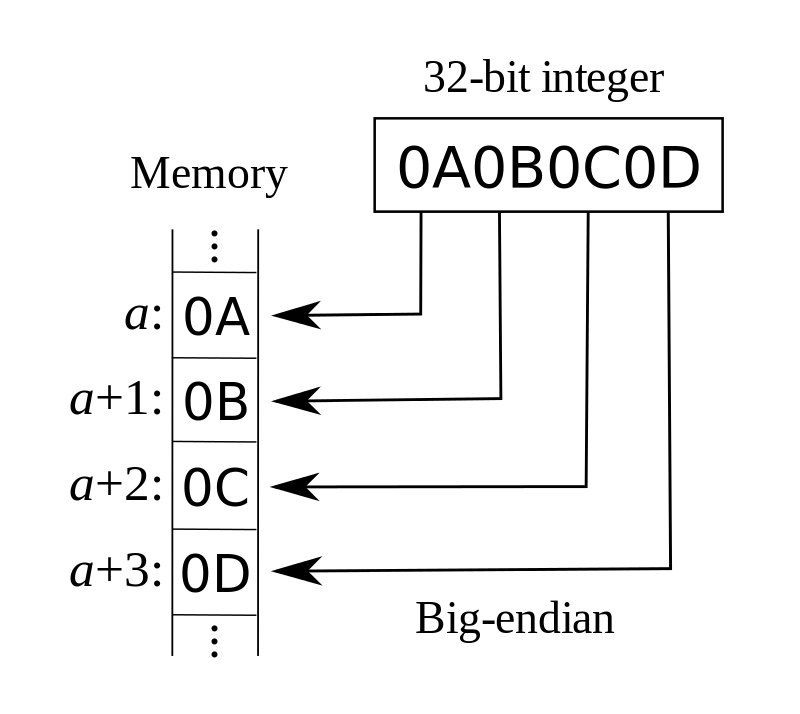
\includegraphics[scale=0.11]{img/endianess1.png}
			        	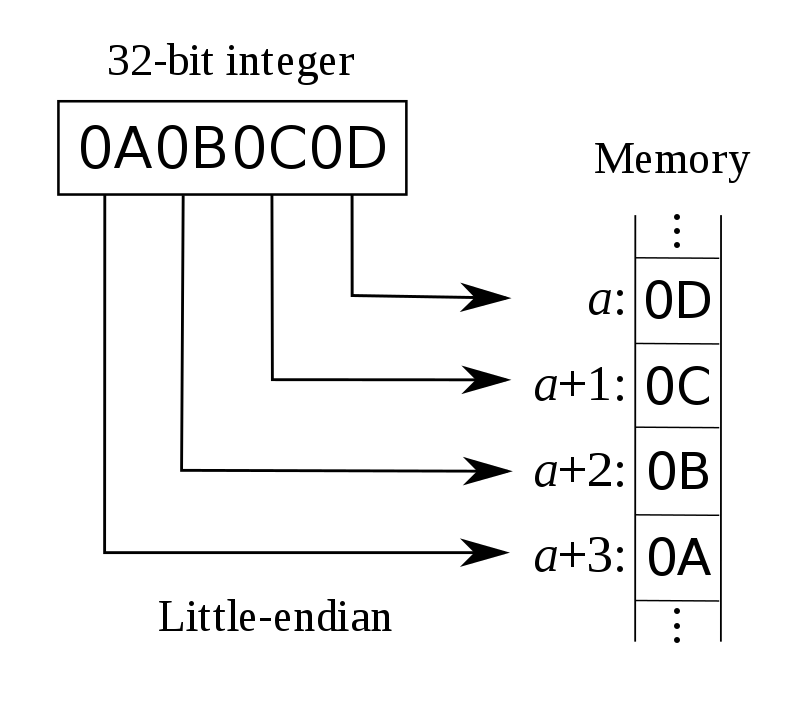
\includegraphics[scale=0.11]{img/endianess2.png}
			    	\end{center}
				\end{column}
			\end{columns}

	    \end{frame}

	    \begin{frame}{La communication}{La sérialisation}

	        \begin{block}{Les messages}
	            Deux types de messages :
	            \begin{itemize}
	                \item Du client au serveur : structure Request\_CTS
	                \item Du serveur au client : structure Request\_STC
	            \end{itemize}
	        \end{block}

	        \begin{block}{Contenu des messages}
	            \begin{itemize}
	                \item Un type enum correspondant au type du message
	                \item Une union des différentes structures de message
	            \end{itemize}
	        \end{block}

	        \begin{block}{Sérialisation de message}
	        	\begin{itemize}
	                \item Sérialisation du type de message.
	                \item Sérialisation des éléments de la structure du message.
	            \end{itemize}            
	        \end{block}
	    \end{frame}

	    \begin{frame}[fragile]{La communication}{La sérialisation}
			\begin{columns}
		        \begin{column}{0.4\textwidth}
		        	\begin{scriptsize}
			    		\begin{verbatim}
						struct CTS_TetrominoPlaced {
						  Tetromino tetro;
						};

						struct Request_CTS{
						  enum Type : uint8_t {
						      TYPE_TETROMINO_PLACED,
						      ...
						  };
						  Type type;
						  union {
						      CTS_TetrominoPlaced tetroMsg;
						      ...
						  };
						};
						\end{verbatim}
					\end{scriptsize}
				\end{column}

				\begin{column}{0.5\textwidth}
					\begin{scriptsize}
			        \begin{block}{\begin{small}Exemple : Placement d'un tetromino\end{small}}
			            \begin{enumerate}
			        	\setlength{\leftmargini}{0pt}
							\item{Serialisation :
								\begin{itemize}
								\begin{scriptsize}
					                \item Request\_CTS.type
					                \item Request\_CTS.tetroMsg
					                \newline \rotatebox[origin=c]{180}{$\Lsh$} CTS\_TetrominoPlaced.tetro
								\end{scriptsize}
					            \end{itemize}
							}
							\item{Récupération des données sérialisées
							\newline \rotatebox[origin=c]{180}{$\Lsh$} Sérialisation de la taille du message}
							\item{Envoi sur la socket}
							\item{Réception}
							\item{Désérialisation de la taille du message}
							\item{Désérialisation :
								\begin{itemize}
								\begin{scriptsize}
					                \item Request\_CTS.type
					                \item Request\_CTS.tetroMsg
					                \newline \rotatebox[origin=c]{180}{$\Lsh$} CTS\_TetrominoPlaced.tetro
					            \end{scriptsize}
					            \end{itemize}}
						\end{enumerate}
			        \end{block}
			        \end{scriptsize}
				\end{column}
			\end{columns}        
	    \end{frame}



















	\section{La jouabilité}
		\subsection{Les structures de données}

			\begin{frame}{La jouabilité}{Les structures de données}	

				\begin{block}{La représentation d'un tetromino}
					\begin{itemize}
						\item type
						\item position abscisse/ordonnée
						\item rotation
						\item matrices<2,4> des différents types de tétromino
					\end{itemize}
				\end{block}

				\begin{columns}
					\begin{column}{0.1\textwidth}
						\begin{center}
							
\includegraphics[scale=0.5]{img/2.png}
						\end{center}
					\end{column}
					\begin{column}{0.1\textwidth}
						\begin{center}
							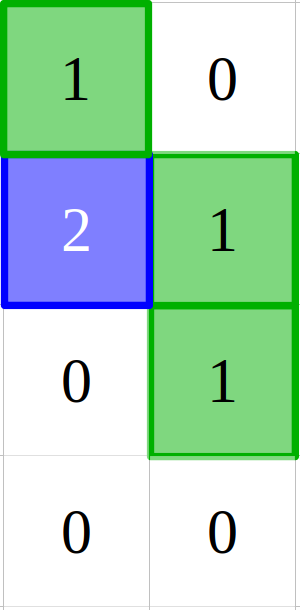
\includegraphics[scale=0.1]{img/tetro.png}
						\end{center}
					\end{column}
				\end{columns}
				
			\end{frame}


			\begin{frame}{La jouabilité}{Les structures de données}	

				\begin{block}{Récupérer les cases à partir de l'ancre}
					\begin{enumerate}
						\item parcours de la matrice
						\item déterminisation de l'ancre
						\item renvoi de la liste de cases occupées par le tétromino
						\item la rotation du tétromino change le sens de parcours
					\end{enumerate}
				\end{block}
				
				\begin{columns}
					\begin{column}{0.1\textwidth}
						\begin{center}
							
\includegraphics[scale=0.5]{img/2.png}
						\end{center}
					\end{column}
					\begin{column}{0.1\textwidth}
						\begin{center}
							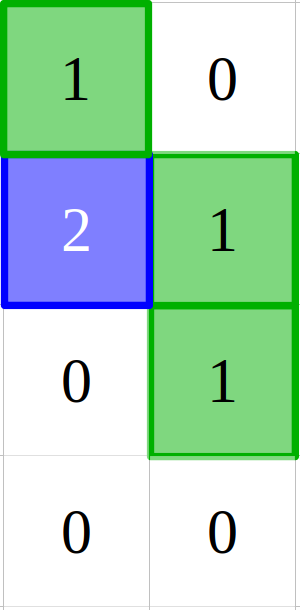
\includegraphics[scale=0.1]{img/tetro.png}
						\end{center}
					\end{column}
				\end{columns}
			\end{frame}

		
			\begin{frame}{La jouabilité}{Les structures de données}
				\begin{columns}
					\begin{column}{0.6\textwidth}
						\begin{block}{La grille permet de vérifier les actions}
							\begin{itemize}
								\item rotation possible
								\item déplacement possible
								\item descente possible
							\end{itemize}
						\end{block}

						\begin{block}{et de vérifier l'état du jeu}
							\begin{itemize}
								\item ligne complète
								\item grille complète
								\item nouveau tétromino en jeu
							\end{itemize}
						\end{block}
					\end{column}
					\begin{column}{0.3\textwidth}
						\begin{center}
							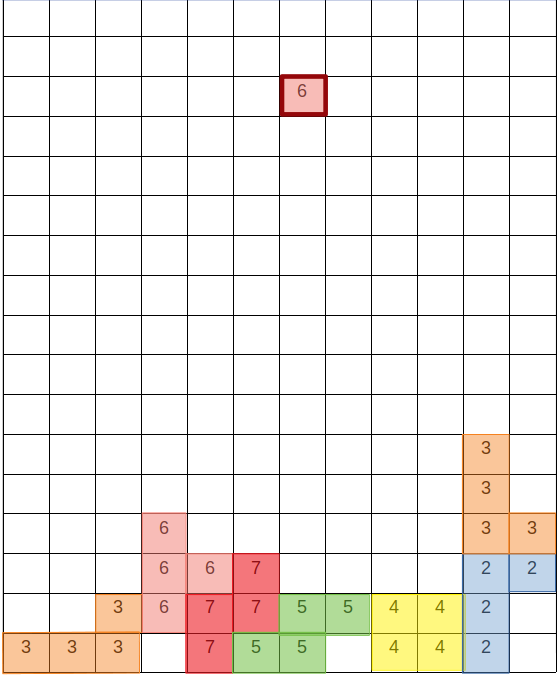
\includegraphics[scale=0.2]{img/gridNB.png}
						\end{center}
					\end{column}
				\end{columns}
			\end{frame}

	\subsection{Le client graphique}

		\begin{frame}{La jouabilité}{Le client graphique}
			\begin{block}{Le rôle du client}
				\begin{itemize}
					\item afficher le jeu
					\item recevoir les messages du serveur
					\item gérer les interactions du joueur
				\end{itemize}
			\end{block}
			\begin{center}
				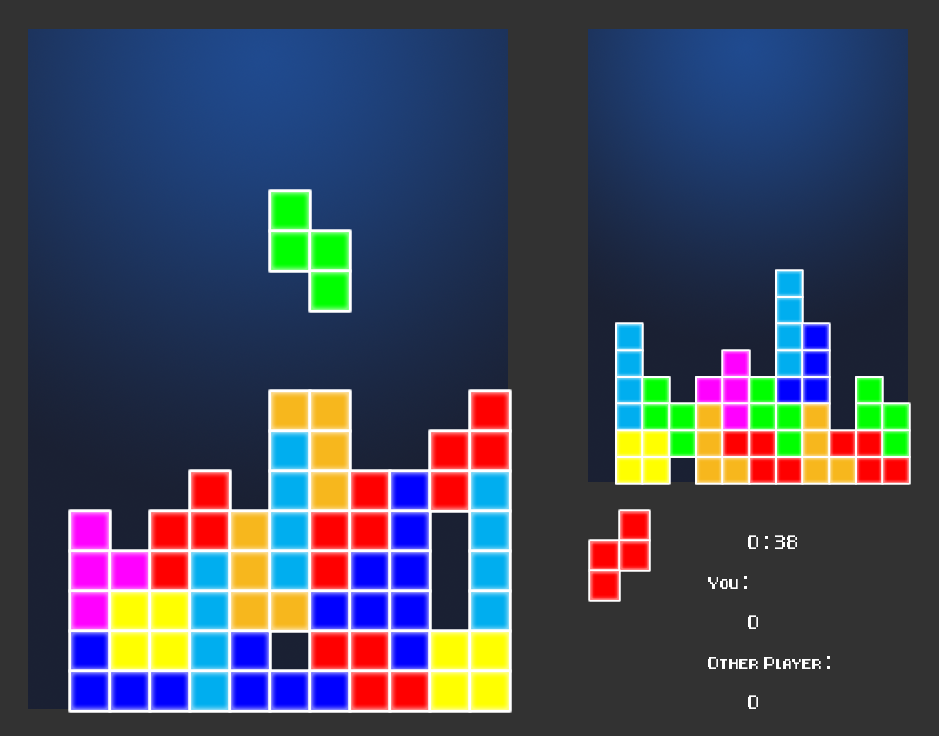
\includegraphics[scale=0.175]{img/vouitris.png}
			\end{center}
		\end{frame}

		\begin{frame}{La jouabilité}{Le client graphique}
			\begin{block}{L'interface}
				\begin{center}
					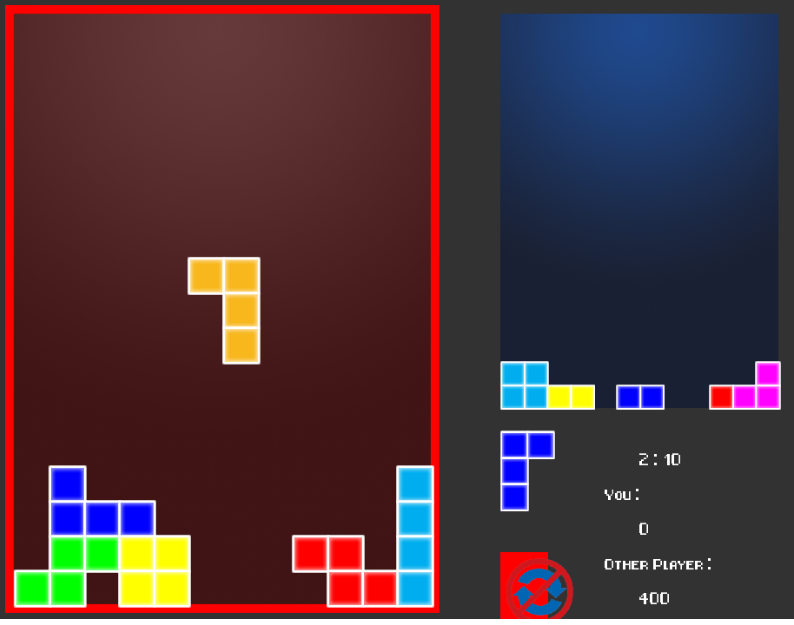
\includegraphics[scale=0.25]{img/bla.png}
				\end{center}
			\end{block}
		\end{frame}

		\begin{frame}{La jouabilité}{Le client graphique}
			\begin{block}{La zone de jeu}
				\begin{center}
					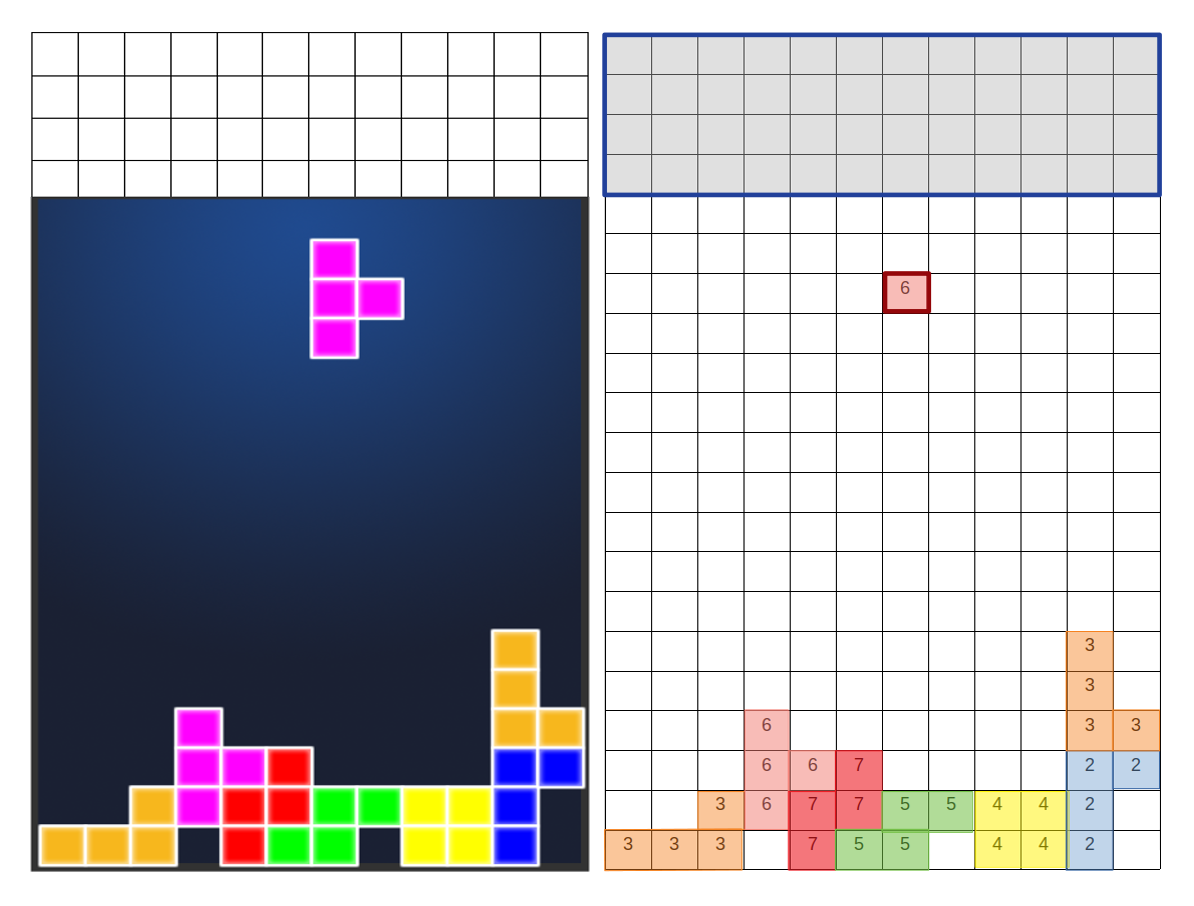
\includegraphics[scale=0.2]{img/grid.png}
				\end{center}
			\end{block}
		\end{frame}


		\begin{frame}{La jouabilité}{Le client graphique}
			\begin{block}{La boucle de jeu}				
				\begin{enumerate}
					\item Vérifier si un message est présent dans la file
						\begin{itemize}
							\item Interpréter le message
						\end{itemize}
					\item Recevoir les actions du joueur
						\begin{itemize}
							\item Vérifier si elles sont possibles
							\begin{itemize}
								\item \'Executer l'action
							\end{itemize}
						\end{itemize}

					\item Vérifier si un tétromino est placé
						\begin{itemize}
							\item Le signaler au serveur
						\end{itemize}

					\item Mettre à jour l'affichage
				\end{enumerate}
			\end{block}
		\end{frame}

		\begin{frame}{La jouabilité}{Le client graphique}
			\begin{block}{L'interprétation des messages}				
				\begin{enumerate}
					\item GameStart
				    	\begin{itemize}
				    		\item Lance l'horloge
				    	\end{itemize}
				   	
				   	\item NewTetromino
				   		\begin{itemize}
				   			\item Place le prochain tétromino en jeu
				   		\end{itemize}

					\item UpdateGrid
				    	\begin{itemize}
				    		\item Met à jour les grilles des joueurs
				    	\end{itemize}

				    \item Malus
				    	\begin{itemize}
				    		\item Applique le malus
				    	\end{itemize}

					\item GameOver
				    	\begin{itemize}
				    		\item Affiche le message de fin
				    	\end{itemize}
				\end{enumerate}
			\end{block}
		\end{frame}

\section*{Conclusion}

		\begin{frame}{Conclusion}
			\begin{block}{Un projet complet...}
				\begin{itemize}
					\item jeu fonctionnel
					\item cahier des charges respecté
				\end{itemize}
			\end{block}

			\begin{block}{...avec des améliorations possibles}
				\begin{itemize}
					\item mode de jeu avec plus de deux joueurs
					\item système anti-triche plus performant
				\end{itemize}
			\end{block}
		\end{frame}

		\begin{frame}{Merci de votre attention}
			\begin{center}
				\Large{Avez-vous des questions ?}
			\end{center}
		\end{frame}




	
\end{document}